% Standalone companion report for the seven-joint Panda implementation.
% The original planar report in ../paper/ is intentionally unchanged.
\documentclass[11pt]{article}

\usepackage[margin=2.35cm]{geometry}
\usepackage{graphicx}
\usepackage{booktabs}
\usepackage{amsmath}
\usepackage{microtype}
\usepackage{placeins}
\usepackage{tabularx}
\usepackage[colorlinks=true,linkcolor=blue]{hyperref}

\graphicspath{{figs/}}
\renewcommand{\topfraction}{0.92}
\renewcommand{\bottomfraction}{0.85}
\renewcommand{\floatpagefraction}{0.75}
\renewcommand{\textfraction}{0.05}
\setlength{\textfloatsep}{13pt plus 3pt minus 3pt}
\newcommand{\vect}[1]{\boldsymbol{#1}}

\title{Contact-Model-Aware Selective Passivation on a 7-DoF Panda\\
\large A Simulation Proof of Concept}
\author{}
\date{}

\begin{document}
\maketitle
\vspace{-1.5em}

\begin{abstract}
This report asks whether selective passivation remains useful when the planar
proof of concept is transferred to a torque-controlled seven-joint robot with
spatial contact ports. In simulation, the Panda maintained a 5-N table contact
while sliding or wiping. Under end-effector blocking, the dual-ledger filter
reduced energy delivered to the human port from 0.263 to 0.049~J. During a
forearm interaction it reduced gross output from 0.158 to 0.060~J while
maintaining contact and 4.26-mm planar RMSE. A reference governor improved
tracking during release without materially changing the protected energy.
The result supports selective, discrete port-energy regulation under the
stated model and known-wrench assumptions; it is not a claim of general human
safety or unconditional robot passivity.
\end{abstract}

\section{Proof-of-concept setup}

The simulated system is a hand-free Franka Panda with seven torque-controlled
joints, a finite pad with four soft contact elements, and a compliant
horizontal table. Control and physics run at 1~kHz. The nominal controller approaches the table, ramps the
normal-force target to 5~N, and then follows either a straight path at
0.03~m/s or a bounded two-dimensional wiping path. A scripted spatial wrench
is applied at a known end-effector or forearm site (Fig.~\ref{fig:setup}). The
known wrench is deliberate: this study isolates the control architecture from
force-estimation uncertainty.

\begin{figure}[!htbp]
  \centering
  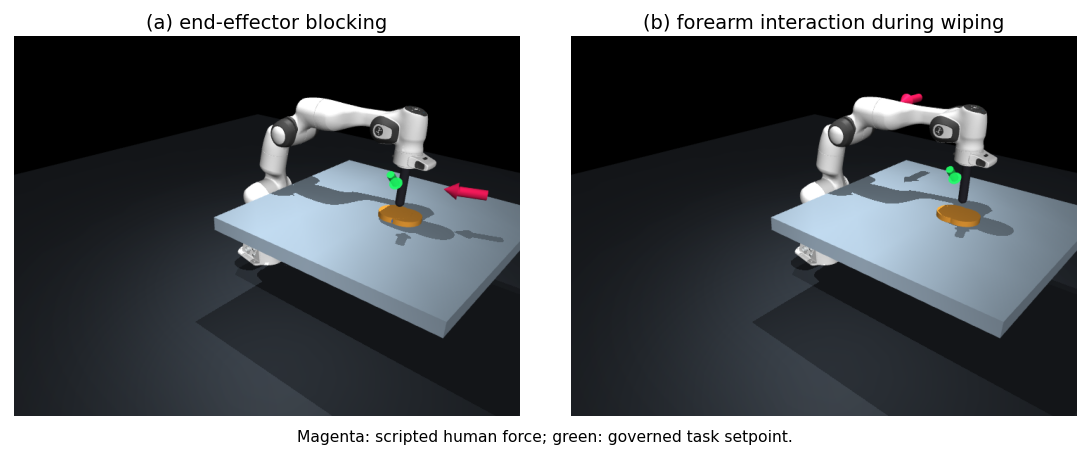
\includegraphics[width=\textwidth]{fig1_setup.png}
  \caption{Panda proof-of-concept tasks during the human-interaction phase.
  The magenta arrow shows the simulator-known human force; the green marker
  shows the governed task setpoint. These markers are visual only.}
  \label{fig:setup}
\end{figure}

Five configurations retain the roles used in the planar report. C3 has no
reference governor; C4 is exactly the C3 filter with the governor enabled.
Consequently, a C3--C4 comparison attributes changes in task behavior to
reference management rather than to a different energy certificate.

\begin{table}[!htbp]
\centering
\caption{Controller configurations.}
\label{tab:modes}
\small
\setlength{\tabcolsep}{5pt}
\begin{tabular}{lllll}
\toprule
Mode & Accounted port & Protected energy & Governor & Role \\
\midrule
C0 & none & none & off & nominal baseline \\
C1 & complete external & $E_W$ & off & whole-port baseline \\
C2 & model residual & $E_R$ & off & model-aware baseline \\
C3 & residual and human & $E_R,E_H$ & off & selective filter \\
C4 & residual and human & $E_R,E_H$ & on & governed C3 \\
\bottomrule
\end{tabular}
\end{table}

\begin{figure}[!htbp]
  \centering
  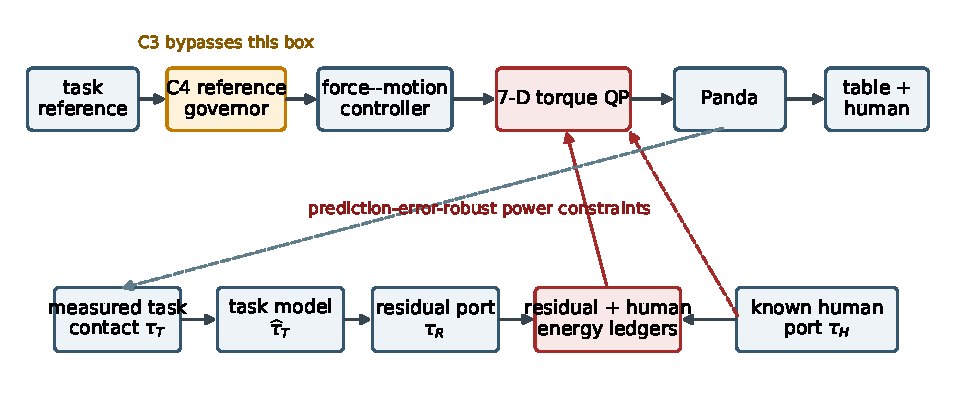
\includegraphics[width=\textwidth]{fig2_architecture.pdf}
  \caption{Controller structure. The QP receives separate residual and human
  accounts. C4 alone modifies the reference upstream of the unchanged C3 QP.}
  \label{fig:architecture}
\end{figure}

\subsection*{Selective-passivation filter}

At each sample, contact and human wrenches are mapped to generalized forces.
The predicted task-contact contribution is removed before accounting:
\begin{equation}
\vect\tau_R=\vect\tau_T+\vect\tau_H-\widehat{\vect\tau}_T,
\qquad
p_i=\vect\tau_i^{\mathsf T}\dot{\vect q},
\quad i\in\{R,H\}.
\end{equation}
Positive power enters the robot. Each ledger uses realized held-sample power,
\begin{equation}
E_{i,k+1}=\min\!\left(E_{i,\max},E_{i,k}+\Delta t\,p_{i,k}^{\rm actual}\right),
\end{equation}
and is not lower-clamped, so a violation remains visible in the log. The
one-step arm-velocity model is affine in the complete applied torque,
\begin{equation}
\dot{\vect q}_{k+1}^{\rm pred}=\vect b_k+\vect B_k\vect\tau,
\qquad
\underline p_i(\vect\tau)=
\vect\tau_i^{\mathsf T}\dot{\vect q}_{k+1}^{\rm pred}
-\lVert\vect\tau_i\rVert\bar e_q .
\end{equation}
The seven-variable QP stays close to the nominal torque and predicted tool
twist while enforcing the residual and, for C3/C4, human-ledger conditions
\begin{equation}
\underline p_i\ge
\max\!\left[
\frac{E_{i,\rm safe}-E_i}{\Delta t},
-k_{\rm cbf}(E_i-E_{i,\rm safe})
\right],
\qquad
\underline p_H\ge-P_H^{\max},
\end{equation}
together with torque, torque-rate, joint-position, and joint-velocity bounds.
The implemented values are $k_{\rm cbf}=8$~s$^{-1}$,
$P_H^{\max}=0.18$~W, $E_H(0)=0.055$~J,
$E_{H,\min}=0.005$~J, and $\bar e_q=0.003$~rad/s. The architecture is
summarized in Fig.~\ref{fig:architecture}.

\FloatBarrier
\section{Proof-of-concept results}

\subsection{Nominal contact and the raw contact signal}

Without human input, both reference motions met the nominal targets
(Table~\ref{tab:nominal}). The compliant-band contact metric was 100\% and no
joint-limit violation occurred. Both this metric and the raw MuJoCo contact
count and force are retained at the 1-ms solver scale. The final pad keeps the
nominal raw constraint continuously active.

\begin{table}[!htbp]
\centering
\caption{Nominal C0 validation during established motion.}
\label{tab:nominal}
\small
\begin{tabular}{lrrrrr}
\toprule
Motion & force RMSE & planar RMSE & orientation RMSE & contact & joint violation \\
 & [N] & [mm] & [deg] & [\%] & \\
\midrule
straight slide & 0.302 & 3.85 & 0.96 & 100 & 0 \\
bounded wipe & 0.378 & 2.91 & 0.67 & 100 & 0 \\
\bottomrule
\end{tabular}
\end{table}

The contact retuning replaced the single sphere with a finite four-element
pad. A 100-ms critically damped contact with low activation-boundary
impedance prevents constraint switching, a 600-ms cosine ramp removes the
tangential velocity step, and a 70-ms causal filter attenuates the small
remaining force variation.
Figure~\ref{fig:smoothing} shows the unfiltered result rather than only the
controller signal. Raw contact occupancy rose from 48.3\% to 100\%, the raw
force peak fell from 12.64 to 5.54~N, and raw-force standard deviation fell
from 5.31 to 0.10~N. Normal-velocity standard deviation fell from 1.49 to
0.175~mm/s. The raw signal is therefore already smooth before filtering.

\begin{figure}[!htbp]
  \centering
  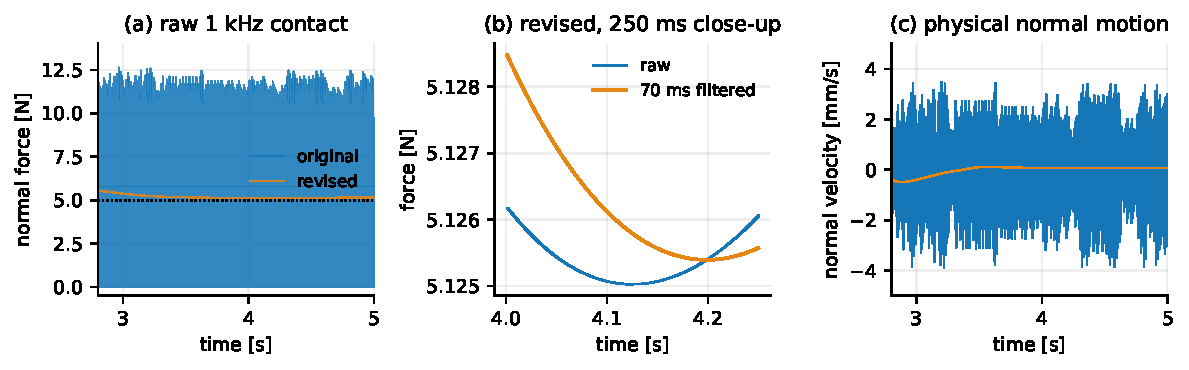
\includegraphics[width=\textwidth]{fig7_smoothing.pdf}
  \caption{Raw contact evidence. (a) The finite pad and soft activation
  boundary remove the unfiltered 1-kHz pulse train. (b) The causal filter
  makes only a small additional change. (c) The revised physical
  normal velocity also has less variation.}
  \label{fig:smoothing}
\end{figure}

\FloatBarrier
\subsection{Model-aware accounting separates task work and mismatch}

In the accurate no-human run, completing the 120-mm slide removed 0.215~J
from C1's whole-port ledger, while C3's residual ledger stayed at 0.300~J
(Fig.~\ref{fig:accounting}a). Both tracked similarly over this finite stroke,
but only C1 spent its budget on expected table friction. With a deliberately
incorrect friction/normal-force predictor, the residual ledger instead fell
by 0.103~J while the human ledger remained exactly at 0.055~J
(Fig.~\ref{fig:accounting}b). Model error is therefore exposed without being
mislabelled as human work.

Whole-port accounting also becomes unreliable when its usable budget is
small. At 0.04, 0.10, and 0.28~J, C1 required 2,077, 1,269, and 1,535 bounded
fallback samples, respectively. These intervals are explicitly uncertified.
At 0.58~J it required no fallback, but allowed the same 0.263~J human output
as C0. This sweep is a limitation of C1, not a successful C1 certificate.

\begin{figure}[!htbp]
  \centering
  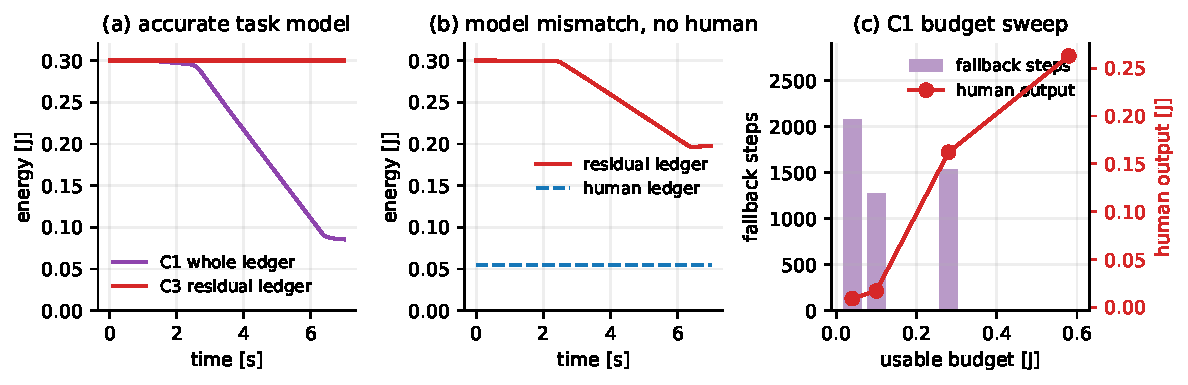
\includegraphics[width=\textwidth]{fig3_accounting.pdf}
  \caption{Why task-aware accounting is needed. (a) Whole-port C1 spends
  energy on ordinary task friction; C3 does not. (b) Predictor mismatch
  appears only in the residual ledger. (c) Small C1 budgets cause fallback,
  whereas a large feasible budget ceases to limit human output.}
  \label{fig:accounting}
\end{figure}

\FloatBarrier
\subsection{The dedicated human port limits transferred energy}

During oblique end-effector blocking, C0 and residual-only C2 each delivered
0.263~J through the human port. C3 reduced this to 0.049~J, close to the
0.050-J usable human-ledger budget, and limited peak output power to 0.148~W
(Fig.~\ref{fig:human}). It did so by slowing and briefly retreating. During
the complete sliding phase, planar RMSE rose to 15.7~mm, force RMSE to
2.87~N, and the maintained-contact fraction fell to 89.6\%. These values expose the intended
safety--task tradeoff rather than suggesting that energy limiting is free.

\begin{figure}[!htbp]
  \centering
  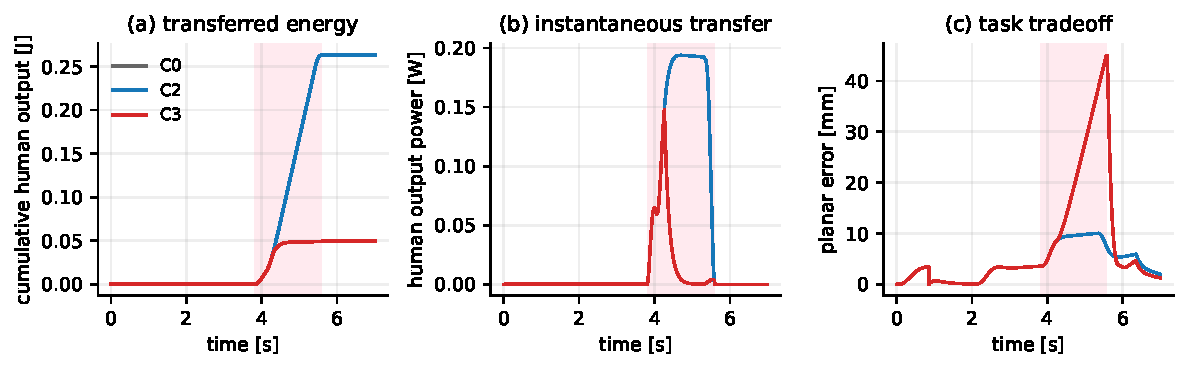
\includegraphics[width=\textwidth]{fig4_human_limiting.pdf}
  \caption{End-effector blocking. The pink region is the human-interaction
  phase. C3 limits transferred energy and power; C0 and C2 do not have the
  dedicated human constraint. The increased tracking error is shown at right.}
  \label{fig:human}
\end{figure}

The forearm experiment tests whether kinematic redundancy can preserve more
of the task while the same human ledger is active. C0 delivered 0.158~J.
C3 admitted 0.010~J of helping input and limited gross output to 0.060~J,
for a net transfer of $-0.049$~J, while maintaining contact and 4.26-mm
planar RMSE (Fig.~\ref{fig:forearm}). Here the arm could reconfigure without
the large task loss seen for direct tool blocking. Under release/recovery,
C3 restored full contact and achieved 1.68-mm planar RMSE over the final
1.5~s.

\begin{figure}[!htbp]
  \centering
  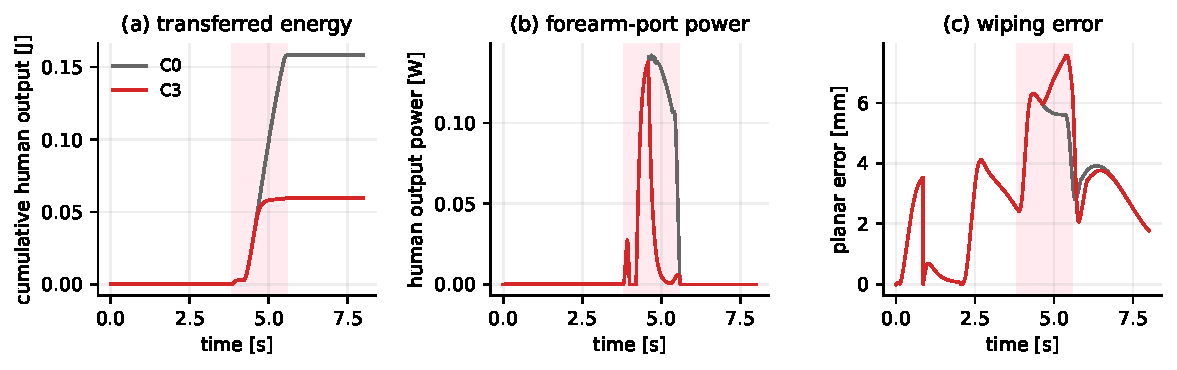
\includegraphics[width=\textwidth]{fig5_forearm.pdf}
  \caption{Forearm interaction during wiping. C3 limits net human extraction
  while using the Panda's redundancy to keep contact and preserve the wiping
  path.}
  \label{fig:forearm}
\end{figure}

\FloatBarrier
\subsection{C4 improves recovery without changing the energy result}

The C3 QP can slow the robot while the original path continues to advance.
C4 smoothly stops that upstream reference while the protected constraint is
active and resumes it after release. Human output was effectively unchanged:
0.04947~J for C3 and 0.04946~J for C4. The governor instead reduced complete-
run planar RMSE from 12.1 to 6.04~mm and raised maintained contact to 99.7\%.
Its maximum progress lag was 44.8~mm and returned to zero after release
(Fig.~\ref{fig:governor}). The safety effect therefore belongs to the QP;
the governor improves how the task reference responds to that intervention.

\begin{figure}[!htbp]
  \centering
  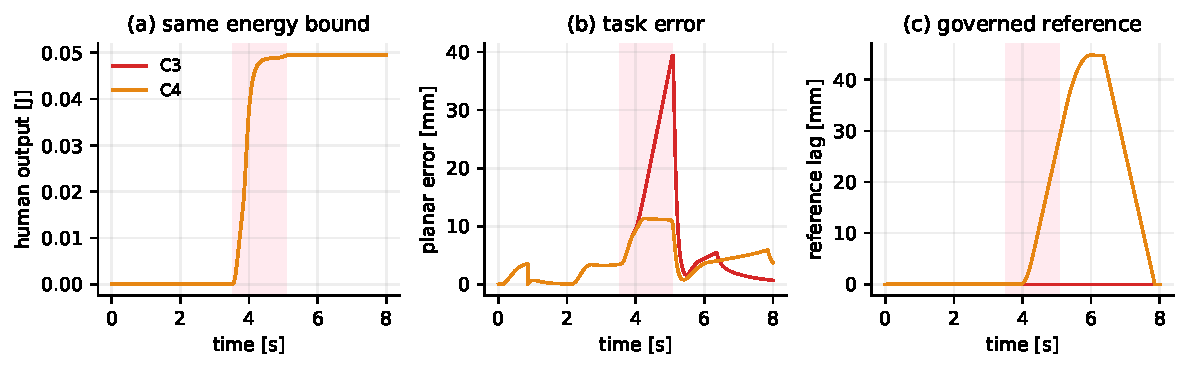
\includegraphics[width=\textwidth]{fig6_governor.pdf}
  \caption{C3 without the governor and C4 with it. Both deliver essentially
  the same bounded human-port energy. C4 temporarily pauses the reference and
  substantially reduces tracking error during interaction and recovery.}
  \label{fig:governor}
\end{figure}

\FloatBarrier
\section{Scope and conclusion}

The frozen one-step velocity-error bound was selected after separate
calibration: the observed calibration maximum was 0.002180~rad/s, compared
with the fixed 0.003~rad/s evaluation bound. The largest C3 evaluation value
was 0.002292~rad/s. Across the focused C3 cases there were zero prediction-
bound violations, protected-energy-floor violations, and QP fallbacks. In
contrast, C1 produced 228 prediction-bound violations across the evaluation
set while operating in its fallback regime; those samples are not presented
as certified behavior.

The work audit also distinguishes the controller ledger from continuous
physical work. The human held-sample versus trapezoidal work discrepancy
stayed below $8.5\times10^{-5}$~J in the focused C3 interactions. The largest
absolute task-contact discrepancy was 0.00649~J. These differences are
reported rather than
absorbed into the certificate.

The Panda study reproduces the planar PoC's central result at a spatial,
seven-joint level: predicted task work can be exempted, model mismatch can be
retained in a residual account, and a dedicated human account can directly
limit energy transfer. It additionally shows that interaction location and
redundancy determine the resulting task cost, and that reference governing
improves recovery without replacing the passivity filter. The evidence
remains conditional on known human wrench and location, the tested predictor,
one-step model accuracy, and numerical QP feasibility. Physical sensing,
continuous-time guarantees, and broader safety validation remain future work.

\end{document}
